% Integrantes:
% - Arthur Gama Ruiz (RA: 23.01445-8)
% - Enzo Oliveira D’Onofrio (RA: 23.01561-6)
% - Felipe Fazio da Costa (RA: 23.00055-4)
% - João Vitor Morimoto Sesma (RA: 23.01516-0)
% - Leonardo Souza Olivieri (RA: 23.01512-8)
% - Pedro Wilian Palumbo Bevilacqua (RA: 23.01307-9)
%
% Data: 04/06/2026
% Matérias: 
% - ECM516_Arquitetura_de_Computadores
% - ECM252_Linguagens_de_Programação_2

\documentclass[aspectratio=169,12pt]{beamer}

% ── Pacotes ──────────────────────────────────────────────────
\usepackage[utf8]{inputenc}
\usepackage[T1]{fontenc}
\usepackage[english]{babel}
\usepackage{helvet}
\renewcommand{\familydefault}{\sfdefault}
\usepackage{tikz}
\usetikzlibrary{shapes.geometric, arrows.meta, fit, positioning, backgrounds, calc}
\usepackage{xcolor}
\usepackage{listings}
\usepackage{booktabs}
\usepackage{array}
\usepackage{colortbl}
\usepackage{graphicx}
\usepackage{microtype}
\usepackage{hyperref}

\hypersetup{pdfauthor={Arthur Gama Ruiz, Enzo Oliveira D'Onofrio, Felipe Fazio da Costa, João Vitor Morimoto Sesma, Leonardo Souza Olivieri, Pedro Wilian Palumbo Bevilacqua}}

% ── Paleta de cores Modern & Clean ────────────────────────────
\definecolor{DeepBlue}{HTML}{0A192F}
\definecolor{AccentBlue}{HTML}{64FFDA}
\definecolor{SlateBlue}{HTML}{112240}
\definecolor{TextGray}{HTML}{8892B0}
\definecolor{White}{HTML}{CCD6F6}
\definecolor{CodeBG}{HTML}{172A45}

% ── Tema Beamer Customizado ──────────────────────────────────
\usetheme{metropolis} % Requer o pacote 'beamerthememetropolis' disponível no TeX Live
\setbeamercolor{normal text}{fg=White, bg=DeepBlue}
\setbeamercolor{alerted text}{fg=AccentBlue}
\setbeamercolor{example text}{fg=AccentBlue}
\setbeamercolor{structure}{fg=AccentBlue}
\setbeamercolor{background canvas}{bg=DeepBlue}
\setbeamercolor{frametitle}{bg=DeepBlue, fg=White}
\setbeamercolor{block title}{bg=SlateBlue, fg=AccentBlue}
\setbeamercolor{block body}{bg=SlateBlue!50, fg=White}

% Ajuste do rodapé
\setbeamertemplate{footline}{%
  \begin{beamercolorbox}[wd=\paperwidth,ht=2.25ex,dp=1ex,right,rightskip=1cm]{normal text}%
    \tiny CEUN-IMT - Instituto Mauá de Tecnologia \quad | \quad \insertframenumber{}/\inserttotalframenumber
  \end{beamercolorbox}%
}

% ── Listings (código) ────────────────────────────────────────
\lstdefinelanguage{JavaScript}{
  morekeywords={async, await, break, case, catch, class, const, continue, debugger, default, delete, do, else, enum, export, extends, false, finally, for, function, if, import, in, instanceof, let, new, null, return, super, switch, this, throw, true, try, typeof, var, void, while, with, yield},
  sensitive=true,
  morecomment=[l]{//},
  morecomment=[s]{/*}{*/},
  morestring=[b]',
  morestring=[b]"
}

\lstset{
  language=JavaScript,
  basicstyle=\ttfamily\tiny\color{White},
  backgroundcolor=\color{CodeBG},
  keywordstyle=\color{AccentBlue}\bfseries,
  commentstyle=\color{TextGray}\itshape,
  stringstyle=\color{AccentBlue!70},
  numberstyle=\tiny\color{TextGray},
  numbers=left,
  numbersep=6pt,
  frame=none,
  breaklines=true,
  showstringspaces=false,
  tabsize=2,
  literate={á}{{\'a}}1 {ã}{{\~a}}1 {é}{{\'e}}1 {í}{{\'i}}1 {ó}{{\'o}}1 {ú}{{\'u}}1 {ç}{{\c{c}}}1 {õ}{{\~o}}1
}

% ── Comandos utilitários ─────────────────────────────────────
\newcommand{\badge}[2]{%
  \tikz[baseline=-3pt]\node[fill=#1, text=DeepBlue, rounded corners=3pt,
    inner xsep=5pt, inner ysep=2pt, font=\bfseries\tiny]{#2};}

% ── Metadados ─────────────────────────────────────────────────
\title{\textbf{SkySwift}}
\subtitle{Infraestrutura de Entrega via Drones}
\author{Arthur Gama Ruiz \and Enzo D'Onofrio \and Felipe Fazio \and Jo\~ao Morimoto \and Leonardo Olivieri \and Pedro Bevilacqua}
\institute{CEUN-IMT - Instituto Mauá de Tecnologia}
\date{2026}

% ============================================================
\begin{document}
% ============================================================

% ── CAPA CORRIGIDA ──────────────────────────────────────────
{
\setbeamertemplate{footline}{}
\begin{frame}[plain]
  \begin{tikzpicture}[remember picture, overlay]
    % Fundo minimalista
    \fill[DeepBlue] (current page.south west) rectangle (current page.north east);
    % Detalhe de linha geométrica
    \draw[AccentBlue!30, line width=1pt] ($(current page.north west) + (1cm,-2cm)$) -- ($(current page.north east) + (-1cm,-2cm)$);
  \end{tikzpicture}
  
  \centering
  \vspace{1 cm}
  {\Huge \textbf{\textcolor{White}{SkySwift}}} \\
  \vspace{0.2cm}
  {\large \textcolor{AccentBlue}{Plataforma de Logística Autônoma via Drones}} \\
  
  \vfill
  
  \begin{columns}[T]
    \column{0.45\textwidth}
      \scriptsize
      \textbf{\textcolor{White}{Desenvolvimento:}} \\
      Arthur Gama Ruiz (23.01445-8) \\
      Enzo O. D’Onofrio (23.01561-6) \\
      Felipe Fazio da Costa (23.00055-4)
    \column{0.45\textwidth}
      \scriptsize
      \textbf{\textcolor{White}{\phantom{Desenvolvimento:}}} \\
      João V. Morimoto Sesma (23.01516-0) \\
      Leonardo S. Olivieri (23.01512-8) \\
      Pedro W. P. Bevilacqua (23.01307-9)
  \end{columns}
  
  \vfill
  
  {\tiny \textcolor{TextGray}{CEUN-IMT - Instituto Mauá de Tecnologia \quad | \quad 2026}}
\end{frame}
}

% ── VISÃO GERAL ──────────────────────────────────────────────
\begin{frame}{01 | Proposta de Valor}
  \begin{itemize}
    \item \textbf{\textcolor{AccentBlue}{Eficiência:}} Redução drástica no tempo de entrega urbana.
    \item \textbf{\textcolor{AccentBlue}{Escalabilidade:}} Arquitetura de microsserviços pronta para crescimento.
    \item \textbf{\textcolor{AccentBlue}{Segurança:}} Comunicação criptografada e autenticação JWT.
  \end{itemize}
  \vfill
  \begin{block}{Objetivo Técnico}
    Integrar conceitos de \textbf{Arquitetura de Computadores (Distributed Processing)} com \textbf{Linguagens de Programação (JavaScript/React)}.
  \end{block}
\end{frame}

% ── ARQUITETURA CLEAN ────────────────────────────────────────
\begin{frame}{02 | Arquitetura de Eventos}
  \centering
  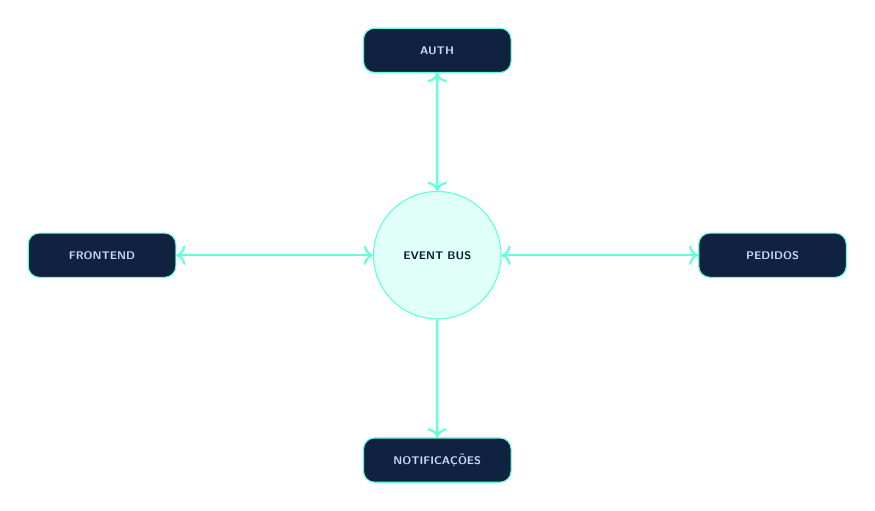
\begin{tikzpicture}[node distance=1.5cm, auto, scale=0.8, every node/.style={scale=0.8}]
    \tikzstyle{svc} = [rectangle, draw=AccentBlue, fill=SlateBlue, text=White, text width=6em, text centered, rounded corners, minimum height=2em, font=\tiny\bfseries]
    \tikzstyle{hub} = [circle, draw=AccentBlue, fill=AccentBlue!20, text=DeepBlue, text width=5em, text centered, font=\tiny\bfseries]
    
    \node [hub] (hub) {EVENT BUS};
    \node [svc, left=2.5cm of hub] (ui) {FRONTEND};
    \node [svc, above=of hub] (auth) {AUTH};
    \node [svc, right=2.5cm of hub] (orders) {PEDIDOS};
    \node [svc, below=of hub] (notify) {NOTIFICAÇÕES};
    
    \draw [AccentBlue, <->, thick] (ui) -- (hub);
    \draw [AccentBlue, <->, thick] (auth) -- (hub);
    \draw [AccentBlue, <->, thick] (orders) -- (hub);
    \draw [AccentBlue, ->, thick] (hub) -- (notify);
  \end{tikzpicture}
  \vfill
  {\tiny \textcolor{TextGray}{Modelo Publish/Subscribe: O emissor nunca conhece o receptor.}}
\end{frame}

% ── CÓDIGO DO BARRAMENTO ─────────────────────────────────────
\begin{frame}[fragile]{03 | Implementação: Broadcast HTTP}
  \begin{lstlisting}[caption=Lógica de Broadcast de Eventos]
async function distribuirEvento(evento) {
  const inscritos = await db.getInscritos(); // Recupera lista de webhooks
  
  await Promise.all(inscritos.map(async (servico) => {
    if (servico.nome === evento.origem) return;

    try {
      await axios.post(`${servico.url}/receber`, evento, { timeout: 5000 });
    } catch (err) {
      console.error(`Falha no broadcast para: ${servico.nome}`);
    }
  }));
}
  \end{lstlisting}
  \vfill
  \badge{AccentBlue}{Event-Driven} \quad \badge{AccentBlue}{Assíncrono}
\end{frame}

% ── SEGURANÇA ────────────────────────────────────────────────
\begin{frame}[fragile]{04 | Backend: Segurança e JWT}
  \begin{columns}[T]
    \column{0.5\textwidth}
      \begin{itemize}
        \item \textbf{Identity Provider:} JWT assinado digitalmente.
        \item \textbf{Privacy:} Hashing \texttt{bcrypt} (10 rounds).
        \item \textbf{Arquitetura:} Stateless (não salva sessão no servidor).
      \end{itemize}
    \column{0.5\textwidth}
      \begin{lstlisting}
// Validação de Token (Middleware)
function autenticar(req, res, next) {
  const token = req.headers['authorization'];
  if (!token) return res.sendStatus(401);
  
  jwt.verify(token, SECRET, (err, user) => {
    if (err) return res.sendStatus(403);
    req.user = user;
    next();
  });
}
      \end{lstlisting}
  \end{columns}
\end{frame}

% ── ROTEAMENTO ───────────────────────────────────────────────
\begin{frame}{05 | Lógica de Roteamento}
  \begin{columns}[T]
    \column{0.5\textwidth}
      \textbf{Fórmula de Haversine} \\
      Utilizada para cálculo de distância geodésica quando APIs externas estão indisponíveis.
      \vspace{0.5cm}
      \begin{equation*}
        a = \sin^2\left(\frac{\Delta\phi}{2}\right) + \cos\phi_1\cos\phi_2\sin^2\left(\frac{\Delta\lambda}{2}\right)
      \end{equation*}
    \column{0.5\textwidth}
      \begin{itemize}
        \item \textbf{Entrada:} Coordenadas GPS (WGS84).
        \item \textbf{Saída:} Distância em metros + ETA (Tempo estimado).
        \item \textbf{Fallback:} Garantia de operação offline.
      \end{itemize}
  \end{columns}
\end{frame}

% ── FRONTEND ─────────────────────────────────────────────────
\begin{frame}{06 | Frontend: React 19 \& UX}
  \begin{itemize}
    \item \textbf{State Management:} Hooks customizados para pedidos e notificações.
    \item \textbf{Modern UX:} Interface otimizada com \textit{Dark Mode} nativo.
    \item \textbf{Performance:} \textit{Vite} como motor de build ultrarrápido.
  \end{itemize}
  \vfill
  \centering
  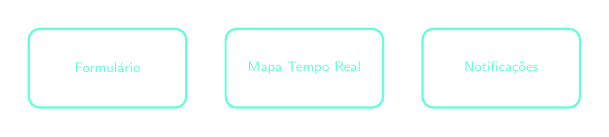
\begin{tikzpicture}
    \draw[AccentBlue, thick, rounded corners] (0,0) rectangle (2,1) node[midway, font=\tiny]{Formulário};
    \draw[AccentBlue, thick, rounded corners] (2.5,0) rectangle (4.5,1) node[midway, font=\tiny]{Mapa Tempo Real};
    \draw[AccentBlue, thick, rounded corners] (5,0) rectangle (7,1) node[midway, font=\tiny]{Notificações};
  \end{tikzpicture}
\end{frame}

% ── INFRAESTRUTURA ───────────────────────────────────────────
\begin{frame}{07 | Persistência Híbrida}
  \centering
  \begin{tabular}{l l l}
    \toprule
    \textbf{Serviço} & \textbf{Banco} & \textbf{Ambiente} \\
    \midrule
    Cadastro & MySQL & Cloud (Production) \\
    Pedidos & SQLite & Serverless (Dev/Vercel) \\
    Notificações & MySQL & Shared Cloud \\
    \bottomrule
  \end{tabular}
  \vfill
  \begin{block}{Consistência Eventual}
    Garantida pelo repasse de mensagens do Barramento de Eventos.
  \end{block}
\end{frame}

% ── CONCLUSÃO ────────────────────────────────────────────────
\begin{frame}{08 | Conclusão}
  \begin{itemize}
    \item \textbf{Sucesso:} 100\% dos microsserviços integrados.
    \item \textbf{Inovação:} Uso de tecnologia de drones simulada com precisão matemática.
    \item \textbf{Legado:} Base de código modular e documentada.
  \end{itemize}
  \vfill
  \centering
  \textcolor{AccentBlue}{\huge \textbf{Entrega Final: SkySwift v1.0}}
\end{frame}

% ── SLIDE FINAL ──────────────────────────────────────────────
{
\setbeamertemplate{footline}{}
\begin{frame}[plain]
  \begin{tikzpicture}[remember picture, overlay]
    \fill[DeepBlue] (current page.south west) rectangle (current page.north east);
  \end{tikzpicture}
  \centering
  {\Huge \textbf{\textcolor{AccentBlue}{Obrigado!}}} \\
  \vspace{0.8cm}
  {\large \textcolor{White}{SkySwift – Entrega Autônoma via Drones}} \\
  \vspace{1cm}
  {\tiny \textcolor{TextGray}{CEUN-IMT - Instituto Mauá de Tecnologia \quad | \quad 2026}}
\end{frame}
}

\end{document}
